\begin{figure}[!hb]
    \centering
    % \includegraphics{}
    a)
    \begin{minipage}{.45\textwidth}
        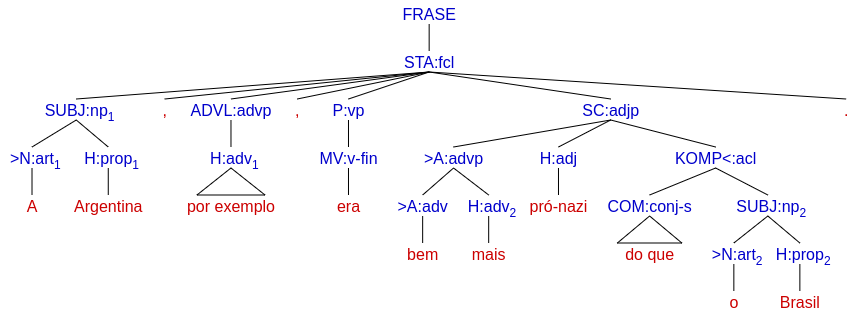
\includegraphics[width=\linewidth]{imagens/ec_bosque_komp_tree_orig.png}
        % \caption{árvore original}
    \end{minipage}
    % 
    b)
    \begin{minipage}{.45\textwidth}
        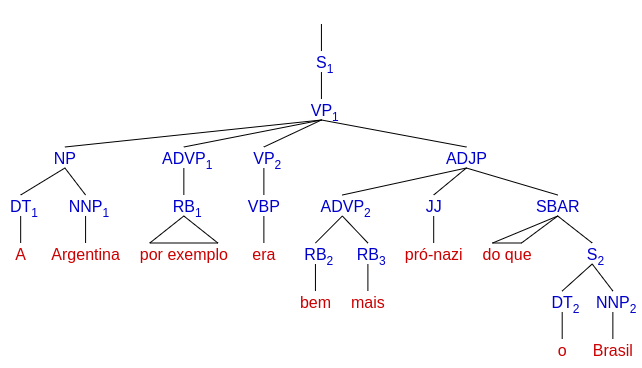
\includegraphics[width=\linewidth]{imagens/ec_bosque_komp_tree_trans.png}
        % \caption{árvore transduzida}
    \end{minipage}
    c)
    \begin{minipage}{.45\textwidth}
        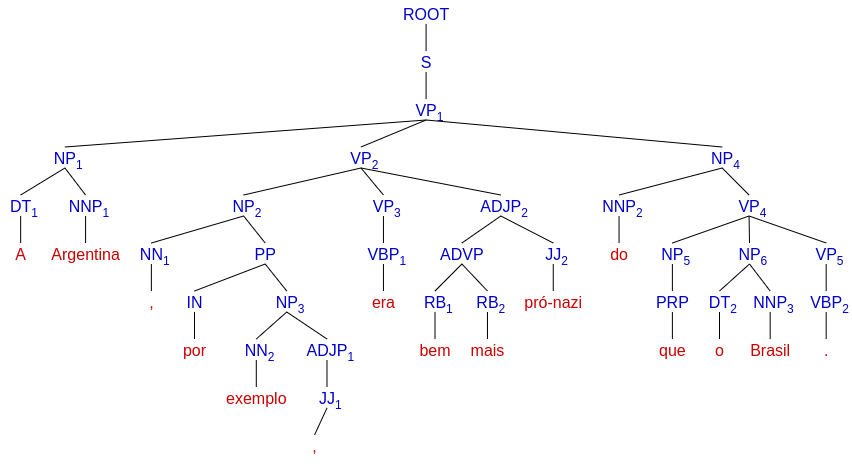
\includegraphics[width=\linewidth]{imagens/ec_bosque_komp_tree_sp.png}
        % \caption{árvore gerada pelo SP}
    \end{minipage}

    \caption[Estudo de caso BOSQUE - Sentença transduzida com KOMP<:acl]{Estudo da sentença CF766-10, \textquote{A Argentina, por exemplo, era bem mais pró-nazi do que o Brasil.}, que possui a estrutura KOMP<:acl internamente. Em a), vemos a árvore relativa à sentença original no BOSQUE. Em b), a sentença pós transdução. E em c), a mesma sentença, classificada pelo SP com uma gramática gerada por este trabalho}
    \label{fig:ec_bosque_komp_tree}
\end{figure}